Date : 19 januari 2024\\

De radiogolf (elektromagnetische golf) ondervindt de volgende verstoringen:
\begin{itemize}
  \item Absorptie: Vooral bij frequenties boven 4 GHz.
  \item Diffractie: Verstoring door objecten in het radiopad.
  \item Obstructie: Onderbreking van het signaal door een object.
  \item Multipath fading: Ongewenste reflecties van het radiosignaal die bij de ontvanger binnenkomen via een andere weg.
  \item Reflecties via ionosfeer en troposfeer (f < 30 MHz).
  \item Free Space Path Loss, vrije ruimte demping.
\end{itemize}

\begin{figure}[H]
    \centering
    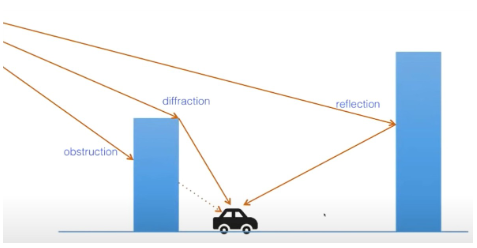
\includegraphics[scale=0.8]{Multipath fading1.png}
    \caption{multipathfading}
    \end{figure}

\begin{figure}[H]
    \centering
    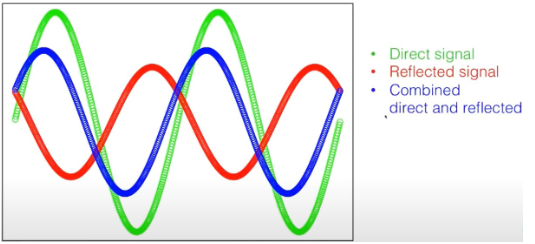
\includegraphics[scale=0.8]{Multipath fading2.png}
    \caption{multipathfading}
    \end{figure}

\begin{figure}[H]
    \centering
    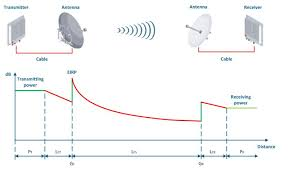
\includegraphics[scale=0.9]{link budget.jpeg}
    \caption{Link Budget}
    \end{figure}

\subsubsection{Free Space Path Loss}

\begin{figure}[H]
    \centering
    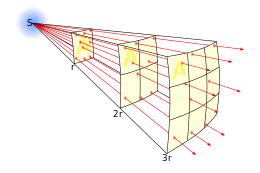
\includegraphics[scale=0.8]{free path space loss.png}
    \caption{free path space loss}
    \end{figure}

Het bereik van een draadloze verbinding wordt in grote mate beperkt door de Free Space Path Loss (FSPL).
\begin{itemize}
    \item Er gaat geen energie verloren, maar de energie verdeelt zich over het oppervlak.
    \item Bij FSPL wordt uitgegaan van een isotrope straler.
    \item Deze antenne straalt het signaal in alle richtingen met gelijke sterkte uit.
\end{itemize}

De Free Space Path Loss (FSPL) formule is gegeven door:

\begin{equation}
\text{FSPL(dB)} = 20 \log_{10}(d) + 20 \log_{10}(f) + 20 \log_{10}\left(\frac{4\pi}{c}\right)
\end{equation}

waarbij:
\begin{align*}
&\text{FSPL(dB)} \text{ is de Free Space Path Loss in decibels} \\
&d \text{ is de afstand tussen de zender en ontvanger in meters} \\
&f \text{ is de frequentie van het signaal in hertz} \\
&c \text{ is de snelheid van het licht in meters per seconde}
\end{align*}

Wat is de FSPL(dB) voor een frequentie van 434 MHz en van 868 MHz op bijv. een afstand van 500 meter?\\
Wat valt je op aan het antwoord?\\
434 MHz = 79,2 dB\\
868 MHz = 85,2 dB\\
Een frequentieverdubbeling leidt tot 6dB (vierdeling) extra demping.

\subsubsection{Antenne}
De antenne zorgt voor: De uitstaling van de radiogolf in de gewenste richting, daardoor mogelijk ook voor compensatie van de FSPL. (De energie wordt gebundeld)\\

Een antenne heeft de volgende kenmerken:
\begin{itemize}
  \item Ingangsimpedantie
  \item Gain en stralingsdiagram (radiation pattern)
  \item Afmeting
  \item Resonantiefrequentie
\end{itemize}

Antenne impedantie

De antenne is te beschouwen als een resonantiekring.
\begin{itemize}
  \item Op de resonantiefrequentie is de impedantie in Ohms. Deze impedantie wordt bepaald door het type antenne en het gebruikte materiaal. Veelvoorkomend is een impedantie van 50 Ohm.
  \item Belangrijk is dat deze impedantie overeenkomt met de feeder (kabel) impedantie en de zender/ontvanger impedantie. Wanneer deze impedantie niet overeenkomt, treedt er reflectie op.
\end{itemize}

\begin{figure}[H]
    \centering
    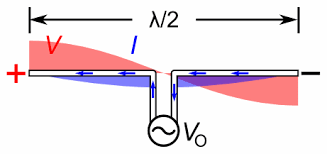
\includegraphics[scale=0.8]{halve golf resonantie.png}
    \caption{De halve golf dipoolantenne in resonantie}
    \end{figure}

We beperken ons tot een veelgebruikt type: de halve golf dipool. De lengte is ongeveer \(0,95 \times \frac{\lambda}{2}\) (de \(0,95\) is de verkortingsfactor van het antennemateriaal).
In een medium is \(\lambda = \frac{c \cdot k}{f}\) (waarbij \(k\) de verkortingsfactor van het materiaal van de antenne is).\\

De polarisatie wordt bepaald door de positie van de straler (dipool),
deze bepaald het elektrische veld.
Typen polarisatie: Horizontaal, verticaal, circulair